% !TEX root = ../lifeonbrane3.tex
%

\section{Brane contributions to generalized entropy}\label{sec:contributions}

In this section we present a modified version of an argument in \cite{Myers:2010tj} which will support our formula for generalized entropy. We consider a geometry with conical defect and rotational symmetry..

adfknadljfalkfj

We separate out the "smooth" contribution of the bulk Riemann tensor away from the conical defect (lying along $\Sigma_b$) via
\beq
^{(\epsilon)}R^{ab}_{\,\,\,\,\,cd} = R^{ab}_{\,\,\,\,\,cd}+2\pi \epsilon \tilde{\varepsilon}^{ab}\tilde{\varepsilon}_{cd}\delta_{\Sigma_b}\,
\eeq where here $\tilde{\varepsilon}$ is the Euclidean volume form spanning the transverse space to $\Sigma_b$ and $R^{ab}_{\,\,\,\,\,cd}$ is the "smooth" piece. The $\delta_{\Sigma_b}$ is a two-dimensional delta function defined in \cite{Myers:2010tj}. The conical singularity runs through the brane so we have a similar decomposition for the Riemann tensor on the brane, $^{(\epsilon)}\tilde{R}^{ab}_{\,\,\,\,\,cd}$, and we denote the intersection of the surface and the brane by $\sigma_b$. The entanglement entropy is computed via \cite{Myers:2010tj}
\beq\label{entropylimit}
S =-\lim_{\epsilon\to0}\Big(\frac{\partial}{\partial \epsilon} + 1\Big) I_{E, 1-\epsilon}\,.
\eeq

The paper \cite{Myers:2010tj} claims it is easy to show the following. The generalization to the brane action should be just as easy \josh{I will verify this.}Note: below I didn't include the two bulk actions because the following section doesn't yet. This will be fixed.
\begin{multline}\label{epsilonaction}
I_{E,1-\epsilon} = (1-\epsilon)I_{E,1} + \int d^{d+1}x \sqrt{g} \Big(\frac{\partial \mathcal{L}_\mt{bulk}}{\partial R^{ab}_{\,\,\,\,\,cd}}\delta_{\Sigma_b} + \frac{\partial \mathcal{L}_\mt{brane}}{\partial \tilde{R}^{ab}_{\,\,\,\,\,cd}}\delta_{\sigma_b}\Big)2\pi \epsilon \tilde{\varepsilon}^{ab}\tilde{\varepsilon}_{cd}+\mathcal{O}(\epsilon^2)\\
=(1-\epsilon)I_{E,1} + 2\pi \epsilon\int d^{d-1}x \sqrt{h}\frac{\partial \mathcal{L}_\mt{bulk}}{\partial R^{ab}_{\,\,\,\,\,cd}} \tilde{\varepsilon}^{ab}\tilde{\varepsilon}_{cd}+ 2\pi \epsilon\int d^{d-2}x \sqrt{h'}\frac{\partial \mathcal{L}_\mt{brane}}{\partial \tilde{R}^{ab}_{\,\,\,\,\,cd}} \tilde{\varepsilon}^{ab}\tilde{\varepsilon}_{cd}+\mathcal{O}(\epsilon^2)\,,
\end{multline} where $h$ and $h'$ are the induced metrics along the sigma curves.
Now we can plug equation (\ref{epsilonaction}) into equation (\ref{entropylimit}), following \cite{Myers:2010tj} to find
\beq
S = -2\pi \frac{\mathcal{L}_\mt{bulk}}{\partial R^{ab}_{\,\,\,\,\,cd}} \tilde{\varepsilon}^{ab}\tilde{\varepsilon}_{cd} \int_{\Sigma_b} d^{d-1}x \sqrt{h}-2\pi \frac{\mathcal{L}_\mt{brane}}{\partial \tilde{R}^{ab}_{\,\,\,\,\,cd}} \tilde{\varepsilon}^{ab}\tilde{\varepsilon}_{cd} \int_{\sigma_b} d^{d-2}x \sqrt{h'}\,.
\eeq We note that upon analytically continuing back to Lorentzian spacetime the transverse volume forms pick up a negative and we get the formula for the generalized entropy (for an Einstein-Hilbert action on the brane and in the bulk),
\beq
S = \frac{A(\Sigma_b)}{4 G_\mt{bulk}}+ \frac{A(\sigma_b)}{4 G_\mt{brane}}\,.
\eeq

\section{`Bubbles' on the brane and stability}\label{sec:bubbles}

Given the formula for the generalised entropy, eq. \eqref{Sgenint}, an interesting possibility arises. Consider taking the limit when the entangling region becomes the entire spacial slice in the CFT...

\begin{figure}[h]
\begin{center}
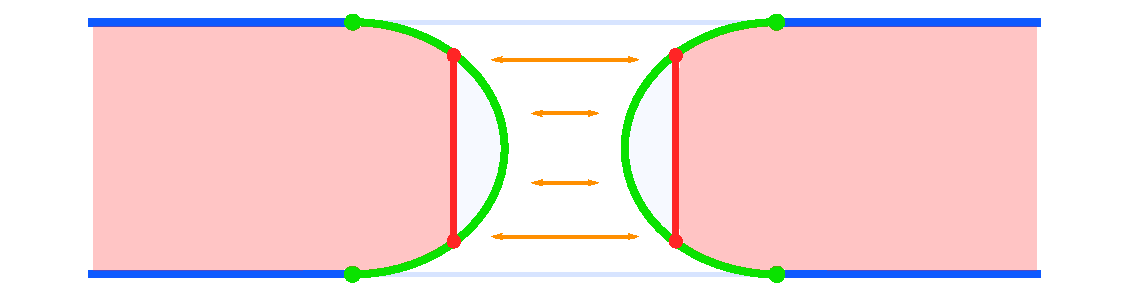
\includegraphics[scale=0.2]{images/bubble} 
\caption{One half of an R-T `bubble' supported on the brane. \iar{Provisional figure...}}
\label{figbubble}
\end{center}
\end{figure}

The generalised entropy of a bubble of radius $P$ is
\begin{align}\label{Agenbubble}
\mathcal{A}_{gen}&=\frac{\pi L^2}{\Gbk} \left(  \sqrt{1+P^2}-1  + \lambda P \right)\ \ ,\ \ \lambda=\frac{\Gbk}{2L \Gbr}
\end{align}

It is illuminating to contrast this with the formula for the effective gravitational constant on the brane, eq. \eqref{Geff}, which can be rewritten in terms of $\lambda$ as
\begin{align}\label{Gefflambda}
\Geff=\frac{\lambda}{1+\lambda}\Gbr
\end{align}

Now recall that we will always consider $\Gbk>0$, but allow for the possibility of $\Gbr$ to become negative, for instance due to quantum corrections. As we will see in short, this has a nice physical interpretation. Note that the function $\lambda/(1+\lambda)$ describes a hyperbola with an asymptote at $\lambda=-1$, being negative for $\lambda>-1$ and positive for $\lambda<-1$.

First let us consider the case $\lambda>0$, which implies $\Gbr>0$ as well. Then, the generalised area function \eqref{Agenbubble} is a monotonically increasing function of $P$, and therefore its minimum lies at $P=0$, where the bubble disappears. Therefore, we find $S_{gen}=0$ for this case. Now, turning to eq. \eqref{Gefflambda}, we see that the effective Newton constant on the brane is positive and finite for $\lambda>0$. This is the `standard' regime where the R-T formula has been explored. 

However, a more interesting scenario is what happens if we allow for negative $\lambda$, which implies $\Gbr<0$ due to eq. \eqref{Agenbubble}. First, for $-1<\lambda<0$, the global minimum of \eqref{Agenbubble} is also a local minimum, corresponding to a bubble of radius $P=-\lambda/\sqrt{1-\lambda^2}$ (notice $P>0$ since $\lambda<0$) with entropy 
\begin{align}\label{Sgenbubble}
S_{gen}= \frac{\pi L^2}{\Gbk} \left( \sqrt{1-\lambda^2} - 1 \right)<0
\end{align}

Although the entropy of the bubble becomes negative, the bubble is \textit{stable} - there is a well defined global minimum. \iar{Add the boundary entropy of the BCFT?}. Moreover, we see that $-1<\lambda<0$ implies $0<\Geff<\infty$ as before, but now owing to the fact that $\Gbr$ is negative. Finally if $\lambda<-1$ the generalised area of the bubble \eqref{Sgenbubble} becomes unbounded from below, and therefore the bubble entropy becomes infinitely negative as it increases in size. This points towards an intrinsic instability of this regime. Indeed, in this case we have $\Geff<0$ which implies that the graviton on the brane will become a ghosts.

\begin{figure}[h]
\begin{center}
\includegraphics[scale=0.4]{images/Abubble} 
\caption{The generalised area \eqref{Agenbubble} for a bubble as a function of its radius. For $\lambda>0$, the area is minimal for vanishing size, whereas for $-1<\lambda<0$ it has a finite size. For $\lambda<-1$, there is no global minimum, signalling an instability of the system.  \iar{Provisional figure...}}
\label{figAbubble}
\end{center}
\end{figure}


\section{Two-dimensional bulk integration}
\josh{The wording is still a but rough but the equations were checked.}
We have the bulk action
\beq
I = \frac{1}{16\pi G} \int d^2x dz \sqrt{-G}\Big(\frac{-4}{L^2}\Big) + \frac{1}{16\pi G}\int d^2x\sqrt{-\tilde{g}}\, 2\mathcal{K}\,,
\eeq where the first integrand came from the cosmological constant plus the $AdS_3$ Ricci scalar. We first expand the bulk metric's determinant:
\beq
\sqrt{-G} = \sqrt{\frac{L^2}{z^2}\Big(\frac{L^2}{z^2} + \frac{1}{2}+\frac{z^2}{16 	L^2}\Big)^2}\sqrt{-g_{AdS_2}}\,.
\eeq
Integrating out the $z$-direction of the bulk action (and ignoring IR divergent terms) gives
\beq
I = \frac{1}{16\pi G}\int d^2x \Big[ \sqrt{-g_{AdS_2}}\Big(\frac{-2L}{s^2}+
\frac{s^2}{8L^3} + \frac{2}{L}\ln\frac{s}{L}\Big) + 2\sqrt{-\tilde{g}}\mathcal{K}\Big]\,.
\eeq
Now we reabsorb several factors into the metric determinant via
\beq
\sqrt{-g_{AdS_2}} = \frac{\sqrt{-\tilde{g}}}{\frac{L^2}{s^2} + \frac{1}{2}+\frac{s^2}{16 	L^2}}\approx\sqrt{-\tilde{g}}\Big(\frac{s^2}{L^2} - \frac{s^4}{2L^4}+\frac{3s^6}{16L^6}\Big)\,,
\eeq and we use the equation for $\mathcal{K}$
\beq
\mathcal{K} = \frac{2}{L}\frac{4L^2 - s^2}{4L^2+s^2}\approx \frac{2}{L} -\frac{s^2}{L^3}+\frac{s^4}{4L^5}\,.
\eeq
Combining these results gives
\beq
I = \frac{1}{16\pi G}\int d^2x \sqrt{-\tilde{g}}\Big[\frac{2}{L}-\frac{s^2}{L^3}+\frac{s^4}{4L^5}+\Big(\frac{2s^2}{L^3}-\frac{s^4}{L^5}\Big)\ln\frac{s}{L} + \mathcal{O}(s^6/L^6)\Big]\,.
\eeq
Now if we consider the action
\beq
I = \frac{1}{16\pi G}\int d^2x\sqrt{-\tilde{g}}\Big[\frac{2}{L}-L \tilde{R}\ln\frac{s}{L} + \frac{L}{2}\tilde{R}-\frac{L^3}{16}\tilde{R}^2+\dots\Big]\,,
\eeq and expand $\tilde{R}$ at small $s$, we get a matching result. Recall that
\beq
\tilde{R} = \frac{-32s^2}{(4L^2+s^2)^2}\approx -\frac{2s^2}{L^4}+\frac{s^4}{L^6} + \mathcal{O}(s^6/L^6)\,.
\eeq



